%
% GNU courseware, XIN YUAN, 2018
%

\section{软件框架}

\frame{
\centerline{\textbf{\Huge{软件框架}}}
}

\frame{\frametitle{种类}
\begin{enumerate}
\item<1-> 驱动程序框架
\item<2-> 服务器端框架
\item<3-> 浏览器框架
\item<4-> 桌面客户端框架
\end{enumerate}
}

\frame{\frametitle{驱动程序框架}
\begin{itemize}
\item<1-> IO回调函数
\item<2-> 驱动程序的各种事件
\item<3-> 中断程序
\item<4-> 内核线程和延迟回调
\end{itemize}
}

\frame{\frametitle{服务器端框架}
\begin{itemize}
\item<1-> 服务器端由前端服务器和后端服务器组成。
\item<2-> 前端服务器运行客户端可访问的服务和反向代理。
\item<3-> 后端服务器运行各种应用服务器,如数据库服务器、聊天服务器、股票服务器、中间件服务器等。
\end{itemize}
}

\frame{\frametitle{服务器程序框架}
\begin{itemize}
\item<1-> 单进程单线程同步IO
\item<2-> 单进程多线程同步IO
\item<3-> 多进程单线程同步IO
\item<4-> 多进程多线程同步IO
\item<5-> 单进程多线程异步IO
\item<6-> 多进程多线程异步IO
\end{itemize}
}

\frame{\frametitle{服务器程序框架}
\begin{itemize}
\item<1-> 单进程单线程事件IO
\item<2-> 多进程单线程事件IO
\item<3-> 单进程多线程事件IO
\item<4-> 多进程多线程事件IO
\end{itemize}
}

\frame{\frametitle{浏览器框架}
\begin{itemize}
\item<1-> IE, chrome, FireFox, …
\item<2-> 脚本程序
\item<3-> HTML5 \& JavaScript \& Websockets
\item<4-> 网页中的虚拟机
\end{itemize}
}

\frame{\frametitle{桌面客户端框架}
\begin{enumerate}
\item<1-> 字符界面的程序
\item<2-> 图形界面的程序
\end{enumerate}
}

\frame{\frametitle{客户端线程模式}
一般采用多线程同步IO的模式。线程之间同步则采用内核对象,或者异步消息/异步信号的机制。
}

\frame{\frametitle{字符界面模式}
一般采用直接的调用函数/方法的方式。
}

\frame{\frametitle{图形界面模式}
与用户界面 (UI) 相关的最大的问题就是大量的凌乱的代码,原因如下:
\begin{enumerate}
\item<1-> 用户界面包含负责的逻辑用于维护界面相关对象;
\item<2-> 其次也包含了应用程序状态的维护。
\end{enumerate}
}

\frame{\frametitle{用户界面的问题}
\begin{enumerate}
\item<1-> 状态 (State),是用户界面最关心的问题之一。
\item<2-> 逻辑 (Logic)
\item<3-> 同步 (Synchronization)
\end{enumerate}
}

\frame{\frametitle{用户界面框架的发展历史}
MVC—>MVP—>MVVM
}

\frame{\frametitle{MVC模式}
即模型-视图-控制器(Model View Controller)模式,
它是最先提出的方案,强制性地使应用程序的输入、处理和输出分开。
}

\frame{\frametitle{MVC模式}
\noindent
\begin{figure}[h]
\centering
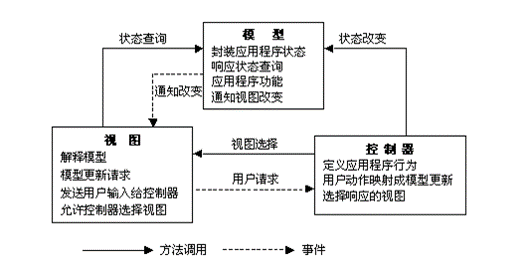
\includegraphics[width=0.9\textwidth]{topics/framework-files/mvc1.png}
\end{figure}
}

\frame{\frametitle{MVC模式}
\noindent
\begin{figure}[h]
\centering
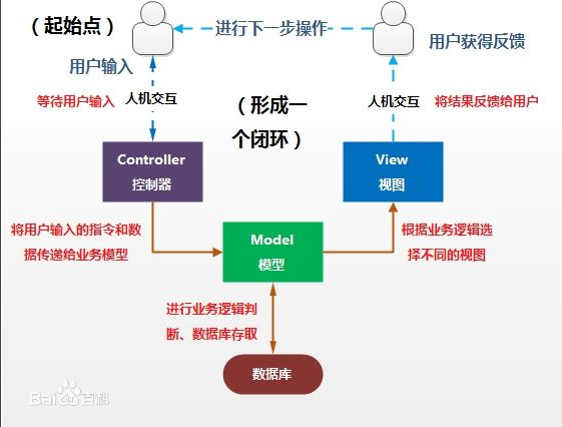
\includegraphics[width=0.8\textwidth]{topics/framework-files/mvc2.png}
\end{figure}
}

\frame{\frametitle{MVC->MVP}
MVC中的Model不是纯粹的Model,因为它要有View的一些数据结构。
M、V、C相互耦合。MVP模式将Model解耦,不再负责View的数据结构。
}

\frame{\frametitle{MVP模式}
MVP是模型-视图-表现类 (Model-View-Presenter) 模式。
}

\frame{\frametitle{MVP模式}
\noindent
\begin{figure}[h]
\centering
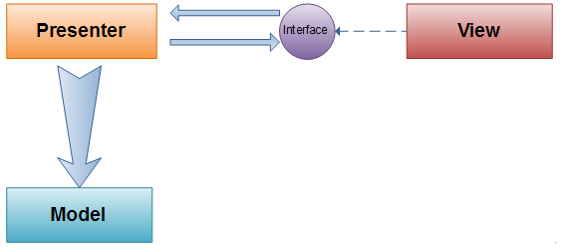
\includegraphics[width=0.9\textwidth]{topics/framework-files/mvp1.png}
\end{figure}
}

\frame{\frametitle{MVP模式}
\noindent
\begin{figure}[h]
\centering
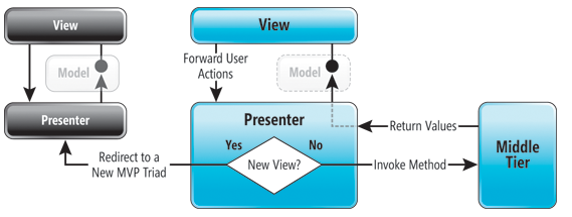
\includegraphics[width=0.9\textwidth]{topics/framework-files/mvp2.png}
\end{figure}
}

\frame{\frametitle{MVP->MVVM}
MVP中的View和Presenter存在耦合。View没有大量的代码逻辑。

~

在C\#的发展过程中,结合WPF、Silverlight的绑定机制,MVP演变为MVVM,
充分利用了WPF、Silverlight的优势,将大量代码逻辑、状态转到ViewModel,
可以说MVVM是专门为WPF、Silverlight打造的。

~

最终,MVVM将View和Presenter解耦。
}

\frame{\frametitle{MVVM模式}
MVVM是模型-视图-视图模型 (Model-View-ViewModel) 模式。
}

\frame{\frametitle{MVVM模式}
\noindent
\begin{figure}[h]
\centering
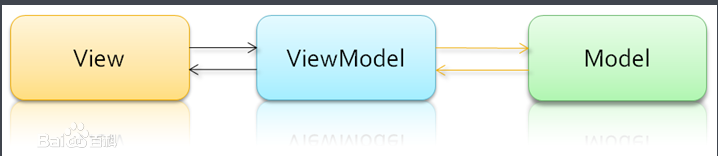
\includegraphics[width=0.9\textwidth]{topics/framework-files/mvvm.png}
\end{figure}
}

\frame{\frametitle{MVVM详解}
MVVM模式由视图(View)、视图模型(ViewModel)、模型(Model)三部分组成,
通过这三部分实现UI逻辑、呈现逻辑和状态控制、数据与业务逻辑的分离。
}

\frame{\frametitle{MVVM详解}
\noindent
\begin{figure}[h]
\centering
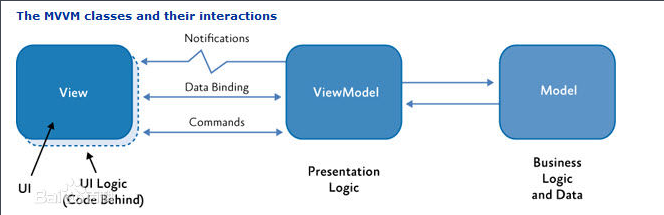
\includegraphics[width=0.9\textwidth]{topics/framework-files/mvvm-detail.png}
\end{figure}
}

\frame{\frametitle{MVVM详解}
\begin{itemize}
\item<1-> View:UI界面。可以是控件容器和集合;
\item<2-> ViewModel:它是View的抽象,负责View与Model之间信息转换,
同时将View的Command传送到Model;
\item<3-> Model:数据访问层,包括业务逻辑。
\end{itemize}
}

\frame{\frametitle{MVVM详解}
View与ViewModel连接:
\begin{enumerate}
\item<1-> Binding Data:数据的绑定
\item<2-> Command:绑定操作的调用
\item<3-> 属性改变的通知
\end{enumerate}
}

\frame{\frametitle{MVVM详解}
ViewModel与Model的连接:
\begin{enumerate}
\item<1-> ViewModel聚合Model对象;
\item<2-> ViewModel直接调用Model的方法;
\item<3-> Model触发事件,ViewModel接收事件。
\end{enumerate}
}

\frame{\frametitle{MVVM优点}
\begin{itemize}
\item<1-> \textbf{低耦合}。视图(View)可以独立于Model变化和修改,
一个ViewModel可以绑定到不同的"View"上,当View变化的时候ViewModel, Model可以不变,
当ViewModel, Model变化的时候View也可以不变。
\item<2-> \textbf{可重用性}。Model可以被聚合到不同的ViewModel中,
ViewModel中的属性命令也可以绑定到不同的View。
\item<3-> \textbf{独立开发}。开发人员可以专注于业务逻辑和数据的开发 (ViewModel和Model),
设计人员可以专注于界面设计和View的开发。
\item<4-> \textbf{可测试}。界面素来是比较难于测试的,而现在单元测试可以针对ViewModel来写。
\end{itemize}
}

\frame{\frametitle{MVVM缺点}
\begin{itemize}
\item<1-> 编写Command的任务重。
\item<2-> ViewModel很容易被误设计为一个界面的活动记录,而不是纯粹的业务逻辑,从而变得庞杂。
\item<3-> 功能和业务逻辑有较大变动时,ViewModel也要做相应的变动。
\item<4-> ViewModel逻辑复用有限。当某个界面上的功能较多时,ViewModel也变得庞大。
而有时为了重用和适用于多个View,ViewModel中还要涉及一些其他View引发的逻辑。
\end{itemize}
}

\frame{\frametitle{MVFM模式}
\begin{enumerate}
\item<1-> 将ViewModel按功能进一步细分,可分为偏向用户界面和偏向数据两个部分。
\item<2-> 偏向数据的部分可进一步按业务逻辑处理的功能细分(最小粒度)为一个或多个功能模型
(Function Model, FM),MVVM模式此时成为MVFM模式。
\item<3-> ViewModel部分可设计为一个或多个ViewModel及FunctionModel,
它们之间可以并列,也可以具有层次性,可通过操纵-事件模式相互关联,
也可通过中介者模式相连。
\end{enumerate}
}

\frame{\frametitle{模式的C++实现}
\noindent
\begin{figure}[h]
\centering
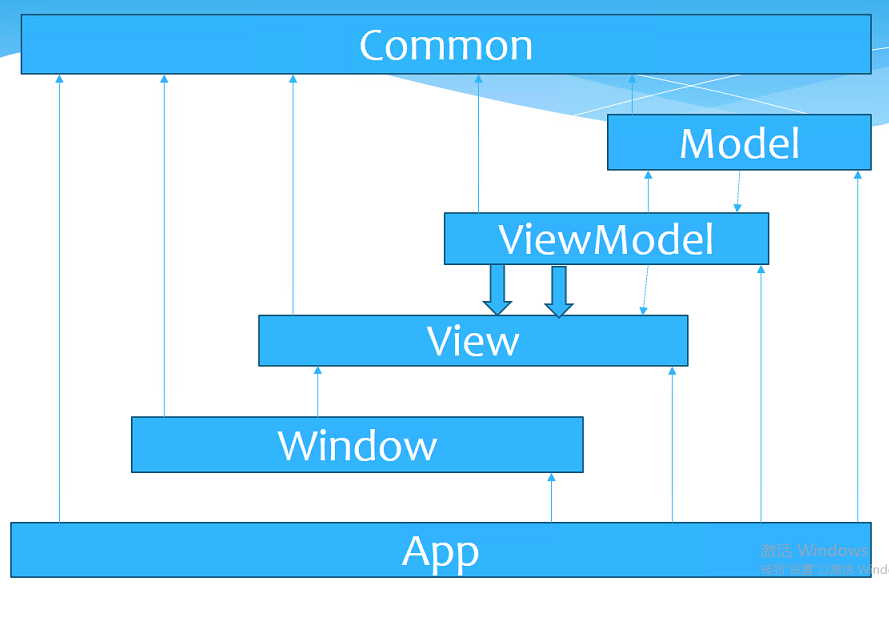
\includegraphics[width=0.8\textwidth]{topics/framework-files/layer.png}
\end{figure}
}

\frame{\frametitle{Common层}
\begin{itemize}
\item<1-> Common层提供基本的类,包括对底层系统的封装,通用性质的数据结构和算法等。
\item<2-> 其它各层都可以调用Common层提供的类。
\end{itemize}
}

\frame{\frametitle{Model层}
\begin{itemize}
\item<1-> 提供应用需要的数据类和业务逻辑的类,提供处理数据的算法类。
\item<2-> 数据类提供属性(用一对get/set方法模拟),方法和事件通知。
\item<3-> 当数据类内部数据发生改变时,发出通知。
\end{itemize}
}

\frame{\frametitle{ViewModel层}
\begin{itemize}
\item<1-> 根据系统中全程需要显示的数据,动态产生并需要显示的数据,
按概念和功能分组,设计多个类。
\item<2-> 聚合Model对象,提供可用来显示的数据类,暴露可用来绑定的数据属性,
暴露可用来绑定的Command对象,提供事件通知(属性改变的通知和Command完成情况的通知)。
\item<3-> 数据类中Command对象在执行体中委托数据类的方法来调用Model层对象的方法。
\item<4-> 当属性发生改变时,触发通知;当命令完成时,触发成功与否的通知。
\end{itemize}
}

\frame{\frametitle{View层}
\begin{itemize}
\item<1-> 实现绘制数据的类和容器类。可以是控件树结构,也可以是场景树结构。
\item<2-> 每个类提供供绑定的属性和命令对象及绑定属性和绑定Command的方法。
\end{itemize}
}

\frame{\frametitle{Window层}
\begin{itemize}
\item<1-> 提供窗口类,聚合View容器对象。
\item<2-> 处理窗口事件,系统输入事件,调用View容器对象的方法来触发Command。
\end{itemize}
}

\frame{\frametitle{App层}
\begin{itemize}
\item<1-> 实现应用装配的类,提供初始化应用的方法,
创建Window、View、ViewModel、Model各层的对象,并将其相互绑定。
\item<2-> 实现消息循环的方法。
\item<3-> 实现Command对象,执行体中可以创建新的一套Window、View、ViewModel、Model各层的对象,
并将其相互绑定。
\end{itemize}
}

\frame{\frametitle{思考}
\begin{enumerate}
\item<1-> 命令模式和undo/redo管理器。
\item<2-> 命令的通知是否有必要?
\end{enumerate}
}

\frame{\frametitle{源代码工程的组织}
\begin{itemize}
\item<1-> 使用智能指针对象来实现绑定,包括通知的绑定。
\item<2-> 每个层放在一个目录下,每个目录下有子目录存放不同类型的类文件。
\end{itemize}
}

\frame{\frametitle{界面程序多线程范式}
\begin{itemize}
\item<1-> 可以在Model层应用多线程编程范式,加速数据处理,使用异步消息/信号机制来触发通知。
\item<2-> 对于2D界面程序,绘制在主线程进行。
\item<3-> 对于3D界面程序,可以在View层应用多线程编程范式,
一般在不是主线程的独立线程进行主要的绘制工作,并可以开启其他线程进行独立的场景绘制。
\end{itemize}
}

\frame{\frametitle{界面库}
\begin{itemize}
\item<1-> MFC, WTL, QT, WxWidget, GTK, FLTK, …
\item<2-> 3D绘制的底层API是DirectX和Vulkan,可以达到最高的绘制性能。
\end{itemize}
}

\frame{\frametitle{两类界面}
\begin{itemize}
\item<1-> 桌面程序具有持续存在的界面,每次交互往往只有部分区域需要更新。
\item<2-> Web应用的页面往往只存在当前的交互中,和本次要更新的数据是一致的。
\end{itemize}
}

\frame{\frametitle{Web界面}
Web应用,即动态网页,可以返回完整的html,也可以通过ajax技术返回部分页面内容,
也可以只返回json数据。无论何种情况,对于服务端的应用程序而言,
数据和界面是一一对应的。所以应用MVC模式就够了。
}

\frame{\frametitle{Web应用}
\begin{itemize}
\item<1-> CGI
\item<2-> FastCGI
\item<3-> Memcached
\item<4-> SCGI
\item<5-> uWSGI (Python)
\end{itemize}
}

\frame{\frametitle{C++开发Web应用}
\begin{itemize}
\item<1-> SCGI
\item<2-> libuv库
\item<3-> MVC模式
\end{itemize}
}

\frame{\frametitle{Web应用的MVC模式}
\begin{itemize}
\item<1-> App层 (绑定Controller对象集合)
\item<2-> Controller层 (提供Controller类和内部的Command对象)
\item<3-> Model层
\item<4-> View层
\item<5-> Command对象绑定Model对象和View对象
\end{itemize}
}

\frame{\frametitle{C++开发Web应用的注意点}
\begin{itemize}
\item<1-> 捕获异常并处理。
\item<2-> 函数必须可重入。
\item<3-> 类成员对象要注意多线程访问的处理。
\item<4-> 尽量使用临时产生的对象并传递。
\end{itemize}
}

\frame{\frametitle{测试框架}
\begin{enumerate}
\item<1-> 可以尝试自行编写一套基于模板类的测试框架。
\item<2-> 使用Lamba表达式作为测试代码体。
\item<3-> 请自行思考:不建议在开发代码中使用Lamba表达式。
\end{enumerate}
}

%end
